%        File: arfc-beamer.tex
%     Created: Sun May 5 10:00 PM 2013 C
%


%\documentclass[11pt,handout]{beamer}
\documentclass[9pt]{beamer}
\usetheme[white]{Illinois}
%\title[short title]{long title}
\title[LEU+ to HALEU Fuel Transitions]{LEU+ to HALEU transitions in advanced reactor fuel cycles}
%\subtitle[short subtitle]{long subtitle}
\subtitle[Short SubTitle]{TWOFCS 2025}
%\author[short name]{long name}
\author[Nathan Ryan]{Nathan S. Ryan$^{*}$, Kathryn D. Huff$^{*}$, Madicken Munk$^{*, \dagger}$}

%\date[short date]{long date}
\date[06.11.2025]{June 11, 2025}
%\institution[short name]{long name}
\institute[UIUC]{$^{*}$Advanced Reactors and Fuel Cycles Group, University of Illinois Urbana-Champaign\\
$^{\dagger}$Scientific Computing, Reactor Analysis and Modeling Group, Oregon State University}

%\usepackage{bbding}
\usepackage{amsfonts}
% \usepackage{algorithm}
% \usepackage[ruled]{algorithm2e}
% \usepackage{algorithmic}
\usepackage{algpseudocode}
% \usepackage{algorithmic}
% \usepackage{array}
\usepackage{amsmath}
\usepackage{xspace}
\usepackage{graphicx}
\usepackage{subfigure}
\usepackage{booktabs} % nice rules for tables
\usepackage{microtype} % if using PDF
\usepackage{bigints}
\usepackage{caption}
\usepackage{xcolor}
\usepackage{tikz}
\usetikzlibrary{positioning, arrows, decorations, shapes, angles, quotes}


\tikzstyle{line} = [draw, -latex']

\definecolor{lightpurple}{HTML}{ECD9ED}
\definecolor{lightgreen}{HTML}{CAE0AB}
\definecolor{lightblue}{HTML}{6D9EEB}


\tikzstyle{block} = [rectangle, draw, fill=lightgreen!20,
    text width=9em, text centered, rounded corners, minimum height=3em]

\newcommand{\cycamore}{\textsc{Cycamore}\xspace}
\newcommand{\cyclus}{\textsc{Cyclus}\xspace}


\newcommand{\units}[1] {\:\text{#1}}%
\newcommand{\SN}{S$_N$}%{S$_\text{N}$}%{$S_N$}%
\DeclareMathOperator{\erf}{erf}
%I need some complimentary error funcitons...
\DeclareMathOperator{\erfc}{erfc}
%Those icons in the references are terrible looking
\setbeamertemplate{bibliography item}[text]


%%%% Acronym support

\usepackage[acronym,toc]{glossaries}
%\newacronym{<++>}{<++>}{<++>}
\newacronym[longplural={metric tons of heavy metal}]{MTHM}{MTHM}{metric ton of heavy metal}
\newacronym{ABM}{ABM}{agent-based modeling}
\newacronym{ACDIS}{ACDIS}{Program in Arms Control \& Domestic and International Security}
\newacronym{AHTR}{AHTR}{Advanced High Temperature Reactor}
\newacronym{ANDRA}{ANDRA}{Agence Nationale pour la gestion des D\'echets RAdioactifs, the French National Agency for Radioactive Waste Management}
\newacronym{ANL}{ANL}{Argonne National Laboratory}
\newacronym{API}{API}{application programming interface}
\newacronym{ARE}{ARE}{Aircraft Reactor Experiment}
\newacronym{ARFC}{ARFC}{Advanced Reactors and Fuel Cycles}
\newacronym{ASME}{ASME}{American Society of Mechanical Engineers}
\newacronym{ATWS}{ATWS}{Anticipated Transient Without Scram}
\newacronym{BDBE}{BDBE}{Beyond Design Basis Event}
\newacronym{BIDS}{BIDS}{Berkeley Institute for Data Science}
\newacronym{CAFCA}{CAFCA}{ Code for Advanced Fuel Cycles Assessment }
\newacronym{CDTN}{CDTN}{Centro de Desenvolvimento da Tecnologia Nuclear}
\newacronym{CEA}{CEA}{Commissariat \`a l'\'Energie Atomique et aux \'Energies Alternatives}
\newacronym{CI}{CI}{continuous integration}
\newacronym{CNEN}{CNEN}{Comiss\~{a}o Nacional de Energia Nuclear}
\newacronym{CNERG}{CNERG}{Computational Nuclear Engineering Research Group}
\newacronym{COSI}{COSI}{Commelini-Sicard}
\newacronym{COTS}{COTS}{commercial, off-the-shelf}
\newacronym{CSNF}{CSNF}{commercial spent nuclear fuel}
\newacronym{CTAH}{CTAHs}{Coiled Tube Air Heaters}
\newacronym{CUBIT}{CUBIT}{CUBIT Geometry and Mesh Generation Toolkit}
\newacronym{CURIE}{CURIE}{Centralized Used Fuel Resource for Information Exchange}
\newacronym{DAG}{DAG}{directed acyclic graph}
\newacronym{DANESS}{DANESS}{Dynamic Analysis of Nuclear Energy System Strategies}
\newacronym{DBE}{DBE}{Design Basis Event}
\newacronym{DESAE}{DESAE}{Dynamic Analysis of Nuclear Energy Systems Strategies}
\newacronym{DHS}{DHS}{Department of Homeland Security}
\newacronym{DOE}{DOE}{Department of Energy}
\newacronym{DRACS}{DRACS}{Direct Reactor Auxiliary Cooling System}
\newacronym{DRE}{DRE}{dynamic resource exchange}
\newacronym{DSNF}{DSNF}{DOE spent nuclear fuel}
\newacronym{DYMOND}{DYMOND}{Dynamic Model of Nuclear Development }
\newacronym{EBS}{EBS}{Engineered Barrier System}
\newacronym{EDZ}{EDZ}{Excavation Disturbed Zone}
\newacronym{EIA}{EIA}{U.S. Energy Information Administration}
\newacronym{EPA}{EPA}{Environmental Protection Agency}
\newacronym{EP}{EP}{Engineering Physics}
\newacronym{FCO}{FCO}{Fuel Cycle Options}
\newacronym{FCT}{FCT}{Fuel Cycle Technology}
\newacronym{FEHM}{FEHM}{Finite Element Heat and Mass Transfer}
\newacronym{FEPs}{FEPs}{Features, Events, and Processes}
\newacronym{FHR}{FHR}{Fluoride-Salt-Cooled High-Temperature Reactor}
\newacronym{FLiBe}{FLiBe}{Fluoride-Lithium-Beryllium}
\newacronym{GDSE}{GDSE}{Generic Disposal System Environment}
\newacronym{GDSM}{GDSM}{Generic Disposal System Model}
\newacronym{GENIUSv1}{GENIUSv1}{Global Evaluation of Nuclear Infrastructure Utilization Scenarios, Version 1}
\newacronym{GENIUSv2}{GENIUSv2}{Global Evaluation of Nuclear Infrastructure Utilization Scenarios, Version 2}
\newacronym{GENIUS}{GENIUS}{Global Evaluation of Nuclear Infrastructure Utilization Scenarios}
\newacronym{GPAM}{GPAM}{Generic Performance Assessment Model}
\newacronym{GRSAC}{GRSAC}{Graphite Reactor Severe Accident Code}
\newacronym{GUI}{GUI}{graphical user interface}
\newacronym{HLW}{HLW}{high level waste}
\newacronym{HPC}{HPC}{high-performance computing}
\newacronym{HTC}{HTC}{high-throughput computing}
\newacronym{HTGR}{HTGR}{High Temperature Gas-Cooled Reactor}
\newacronym{IAEA}{IAEA}{International Atomic Energy Agency}
\newacronym{IEMA}{IEMA}{Illinois Emergency Mangament Agency}
\newacronym{INL}{INL}{Idaho National Laboratory}
\newacronym{IPRR1}{IRP-R1}{Instituto de Pesquisas Radioativas Reator 1}
\newacronym{IRP}{IRP}{Integrated Research Project}
\newacronym{ISFSI}{ISFSI}{Independent Spent Fuel Storage Installation}
\newacronym{ISRG}{ISRG}{Independent Student Research Group}
\newacronym{JFNK}{JFNK}{Jacobian-Free Newton Krylov}
\newacronym{LANL}{LANL}{Los Alamos National Laboratory}
\newacronym{LBNL}{LBNL}{Lawrence Berkeley National Laboratory}
\newacronym{LCOE}{LCOE}{levelized cost of electricity}
\newacronym{LDRD}{LDRD}{laboratory directed research and development}
\newacronym{LFR}{LFR}{Lead-Cooled Fast Reactor}
\newacronym{LLNL}{LLNL}{Lawrence Livermore National Laboratory}
\newacronym{LMFBR}{LMFBR}{Liquid Metal Fast Breeder Reactor}
\newacronym{LOFC}{LOFC}{Loss of Forced Cooling}
\newacronym{LOHS}{LOHS}{Loss of Heat Sink}
\newacronym{LOLA}{LOLA}{Loss of Large Area}
\newacronym{LP}{LP}{linear program}
\newacronym{MA}{MA}{minor actinide}
\newacronym{MCNP}{MCNP}{Monte Carlo N-Particle code}
\newacronym{MILP}{MILP}{mixed-integer linear program}
\newacronym{MIT}{MIT}{the Massachusetts Institute of Technology}
\newacronym{MOAB}{MOAB}{Mesh-Oriented datABase}
\newacronym{MOOSE}{MOOSE}{Multiphysics Object-Oriented Simulation Environment}
\newacronym{MOX}{MOX}{mixed oxide}
\newacronym{MSBR}{MSBR}{Molten Salt Breeder Reactor}
\newacronym{MSRE}{MSRE}{Molten Salt Reactor Experiment}
\newacronym{MSR}{MSR}{Molten Salt Reactor}
\newacronym{NAGRA}{NAGRA}{National Cooperative for the Disposal of Radioactive Waste}
\newacronym{NEAMS}{NEAMS}{Nuclear Engineering Advanced Modeling and Simulation}
\newacronym{NEUP}{NEUP}{Nuclear Energy University Programs}
\newacronym{NFCSim}{NFCSim}{Nuclear Fuel Cycle Simulator}
\newacronym{NGNP}{NGNP}{Next Generation Nuclear Plant}
\newacronym{NMWPC}{NMWPC}{Nuclear MW Per Capita}
\newacronym{NNSA}{NNSA}{National Nuclear Security Administration}
\newacronym{NPRE}{NPRE}{Department of Nuclear, Plasma, and Radiological Engineering}
\newacronym{NQA1}{NQA-1}{Nuclear Quality Assurance - 1}
\newacronym{NRC}{NRC}{Nuclear Regulatory Commission}
\newacronym{NSF}{NSF}{National Science Foundation}
\newacronym{NSSC}{NSSC}{Nuclear Science and Security Consortium}
\newacronym{NUWASTE}{NUWASTE}{Nuclear Waste Assessment System for Technical Evaluation}
\newacronym{NWF}{NWF}{Nuclear Waste Fund}
\newacronym{NWTRB}{NWTRB}{Nuclear Waste Technical Review Board}
\newacronym{OCRWM}{OCRWM}{Office of Civilian Radioactive Waste Management}
\newacronym{ORION}{ORION}{ORION}
\newacronym{ORNL}{ORNL}{Oak Ridge National Laboratory}
\newacronym{PARCS}{PARCS}{Purdue Advanced Reactor Core Simulator}
\newacronym{PBAHTR}{PB-AHTR}{Pebble Bed Advanced High Temperature Reactor}
\newacronym{PBFHR}{PB-FHR}{Pebble-Bed Fluoride-Salt-Cooled High-Temperature Reactor}
\newacronym{PEI}{PEI}{Peak Environmental Impact}
\newacronym{PH}{PRONGHORN}{PRONGHORN}
\newacronym{PRKE}{PRKE}{Point Reactor Kinetics Equations}
\newacronym{PSPG}{PSPG}{Pressure-Stabilizing/Petrov-Galerkin}
\newacronym{PWAR}{PWAR}{Pratt and Whitney Aircraft Reactor}
\newacronym{PWR}{PWR}{Pressurized Water Reactor}
\newacronym{PyNE}{PyNE}{Python toolkit for Nuclear Engineering}
\newacronym{PyRK}{PyRK}{Python for Reactor Kinetics}
\newacronym{QA}{QA}{quality assurance}
\newacronym{RDD}{RD\&D}{Research Development and Demonstration}
\newacronym{RD}{R\&D}{Research and Development}
\newacronym{RELAP}{RELAP}{Reactor Excursion and Leak Analysis Program}
\newacronym{RIA}{RIA}{Reactivity Insertion Accident}
\newacronym{RIF}{RIF}{Region-Institution-Facility}
\newacronym{SFR}{SFR}{Sodium-Cooled Fast Reactor}
\newacronym{SINDAG}{SINDA{\textbackslash}G}{Systems Improved Numerical Differencing Analyzer $\backslash$ Gaski}
\newacronym{SKB}{SKB}{Svensk K\"{a}rnbr\"{a}nslehantering AB}
\newacronym{SNF}{SNF}{spent nuclear fuel}
\newacronym{SNL}{SNL}{Sandia National Laboratory}
\newacronym{STC}{STC}{specific temperature change}
\newacronym{SUPG}{SUPG}{Streamline-Upwind/Petrov-Galerkin}
\newacronym{SWF}{SWF}{Separations and Waste Forms}
\newacronym{SWU}{SWU}{Separative Work Unit}
\newacronym{TRIGA}{TRIGA}{Training Research Isotope General Atomic}
\newacronym{TRISO}{TRISO}{Tristructural Isotropic}
\newacronym{TSM}{TSM}{Total System Model}
\newacronym{TSPA}{TSPA}{Total System Performance Assessment for the Yucca Mountain License Application}
\newacronym{ThOX}{ThOX}{thorium oxide}
\newacronym{UFD}{UFD}{Used Fuel Disposition}
\newacronym{UML}{UML}{Unified Modeling Language}
\newacronym{UOX}{UOX}{uranium oxide}
\newacronym{UQ}{UQ}{uncertainty quantification}
\newacronym{US}{US}{United States}
\newacronym{UW}{UW}{University of Wisconsin}
\newacronym{VISION}{VISION}{the Verifiable Fuel Cycle Simulation Model}
\newacronym{VV}{V\&V}{verification and validation}
\newacronym{WIPP}{WIPP}{Waste Isolation Pilot Plant}
\newacronym{YMR}{YMR}{Yucca Mountain Repository Site}


\makeglossaries

%try to get rid of header on title page\dots
\makeatletter
    \newenvironment{withoutheadline}{
        \setbeamertemplate{headline}[default]
        \def\beamer@entrycode{\vspace*{-\headheight}}
    }{}
\makeatother

% \makeatother
% \setbeamertemplate{footline}
% {
%   \leavevmode%
%   \hbox{%
%     \rightline{\insertframenumber{} / \inserttotalframenumber\hspace*{1ex}}
%   }%
%   \vskip0pt%
% }
% \makeatletter

\setbeamertemplate{caption}{\raggedright\insertcaption\par}
\setbeamertemplate{page number in head/foot}[appendixframenumber]
\setbeamertemplate{caption}[numbered]

\begin{document}
%%%%%%%%%%%%%%%%%%%%%%%%%%%%%%%%%%%%%%%%%%%%%%%%%%%%%%%%%%%%%
%% From uw-beamer Here's a handy bit of code to place at
%% the beginning of your presentation (after \begin{document}):
\newcommand*{\alphabet}{ABCDEFGHIJKLMNOPQRSTUVWXYZabcdefghijklmnopqrstuvwxyz}
\newlength{\highlightheight}
\newlength{\highlightdepth}
\newlength{\highlightmargin}
\setlength{\highlightmargin}{2pt}
\settoheight{\highlightheight}{\alphabet}
\settodepth{\highlightdepth}{\alphabet}
\addtolength{\highlightheight}{\highlightmargin}
\addtolength{\highlightdepth}{\highlightmargin}
\addtolength{\highlightheight}{\highlightdepth}
\newcommand*{\Highlight}{\rlap{\textcolor{HighlightBackground}{\rule[-\highlightdepth]{\linewidth}{\highlightheight}}}}
%%%%%%%%%%%%%%%%%%%%%%%%%%%%%%%%%%%%%%%%%%%%%%%%%%%%%%%%%%%%%
%%--------------------------------%%
\begin{withoutheadline}
\frame{
  \titlepage
}
\end{withoutheadline}

%%--------------------------------%%
\AtBeginSection[]{
\begin{frame}
  \frametitle{Outline}
  \tableofcontents[currentsection]
\end{frame}
}
\begin{frame}
  \frametitle{Know how to code?}
  Consider volunteering in lessons or mentoring in the Computational Resource Access NEtwork (CRANE) so we can support more students!
  \begin{figure}
      \centering
      
\includegraphics[width=0.65\textwidth]{../images/CRANE_logo_inverted.png}
  \end{figure}
  Go to our website: \url{https://www.cranephysics.org}
\end{frame}

% \section{Nuclear Fuel Cycle}
%   \begin{frame}
%       \frametitle{Generally, fuel cycles have these steps}
%       \begin{figure}[ht!]
%       \centering
%       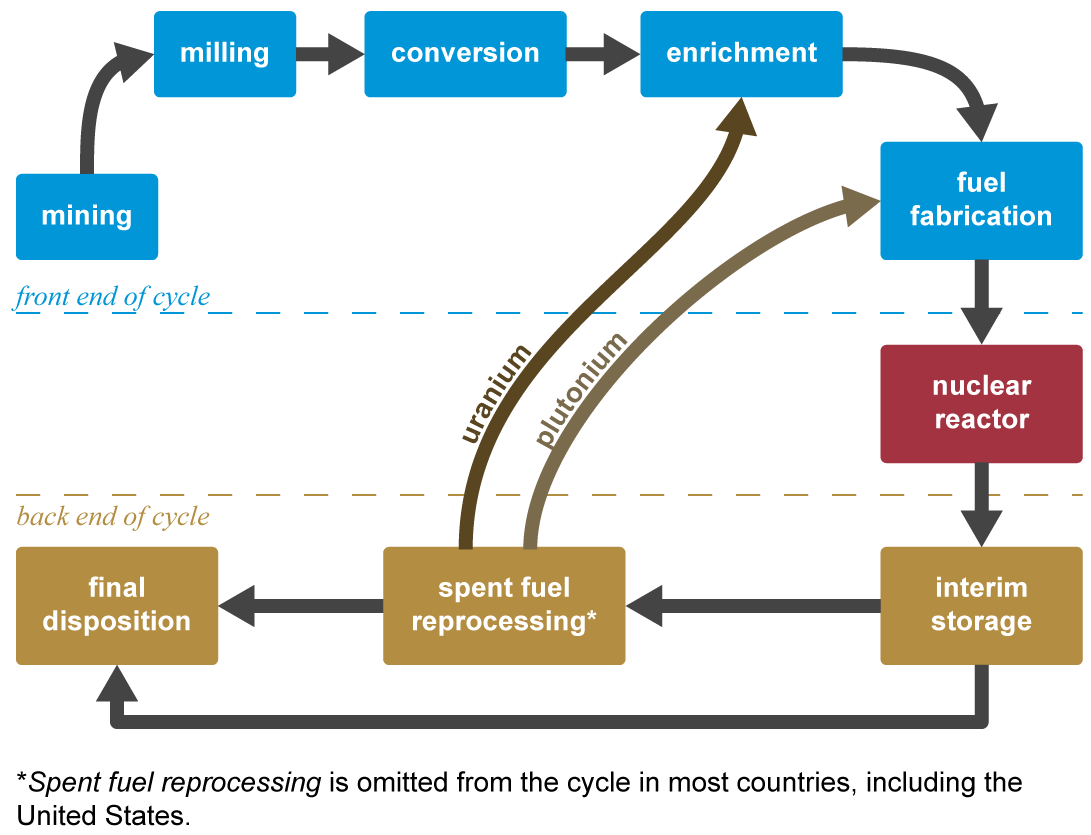
\includegraphics[width=0.75\textwidth]{../images/nuclear_fuel_cycle.png}
%       \caption{Source: Penn State Univ. Radiation Science and Engineering Center (public domain)$^{*}$}
%       \end{figure}
%   \end{frame}

%   \begin{frame}
%       \frametitle{Not all fuel cycles are made equal, and we want options}
%       Concerns about economics, waste generation, proliferation risk, and sustainability motivate the need for fuel cycle options. With metrics like:
%         \begin{itemize}%[<+->]
%             \item natural resource utilization,
%             \item waste mass/volume,
%             \item special material quantities,
%             \item separative work units,
%             \item and energy production,
%         \end{itemize}
%         we can begin to evaluate the tradeoffs between fuel cycle options.
%   \end{frame}

\section{Background}
%   \begin{frame}
%     \frametitle{Big questions in fuel cycle modeling}
%     Increased computational power and advanced reactors mean more detailed fuel cycle modeling.
%     \begin{itemize}
%         \item How can we make facility models more accurate?
%         \item How can we make transaction models more detailed?
%         \item Can we implement nuclear fuel cycle codes to identify realtime diversion or diversion paths?
%         \item When do advanced reactor technologies change key metrics we use to evaluate fuel cycles?
%     \end{itemize}
%   \end{frame}

\begin{frame}
  \frametitle{We use \cyclus to model fuel cycles.}
  \vspace{10pt}
  \cyclus is an open-source agent-based fuel cycle code allowing for detailed facility and transaction modeling \cite{huff_fundamental_2016}.
  % \vspace{10pt}
  \begin{center}
  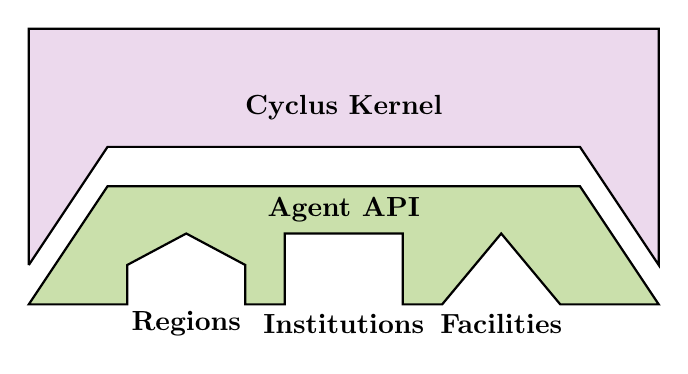
\begin{tikzpicture}
      % Main rectangle
      \draw[thick, fill=lightpurple] (0,0) -- (1,1.5) -- (7, 1.5) -- (8,0) -- (8,3) -- (0,3) -- (0,0);
      \node at (4,2) {\textbf{Cyclus Kernel}};

      % Trapezoid cut-out at the bottom
      \draw[thick, fill=lightgreen] (0,-0.5) -- (1,1) -- (7,1) -- (8,-0.5) -- (6.75, -0.5) -- (6, 0.4) -- (5.25, -0.5) -- (4.75, -0.5) -- (4.75, 0.4) -- (3.25, 0.4) -- (3.25, -0.5) -- (2.75, -0.5) -- (2.75, 0.0) -- (2, 0.4) -- (1.25, 0.0) -- (1.25, -0.5) -- cycle;
      \node at (4,0.7) {\textbf{Agent API}};
      \node at (2, -0.75) {\textbf{Regions}};
      % \node at (2, -1.1) {\textbf{API}};

      \node at (4, -0.75) {\textbf{Institutions}};
      % \node at (4, -1.1) {\textbf{API}};

      \node at (6, -0.75) {\textbf{Facilities}};
      % \node at (6, -1.1) {\textbf{API}};
    \end{tikzpicture}
  \end{center} % \pause

  The \cyclus ecosystem has many \textit{archetypes}, or generic facility models, (like the \cycamore Reactor) that can be used to model different fuel cycle facilities.
  \end{frame}

  \begin{frame}
    \frametitle{What are our options if we cannot get HALEU fuel?}
    \begin{figure}
        \centering
        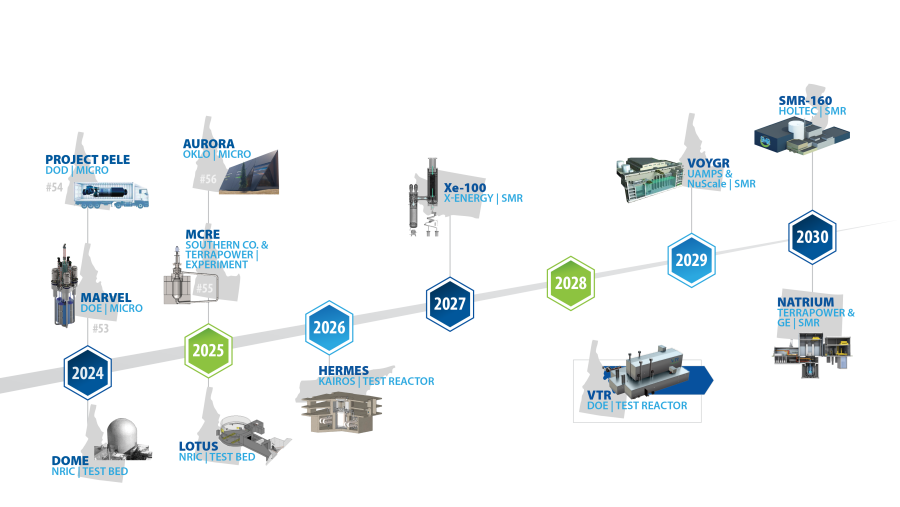
\includegraphics[width=0.86\textwidth]{../images/reactor_timeline.png}
        \caption{Advanced reactor demonstration and deployment projects \cite{inl_reactor_timeline}.}
    \end{figure}
    Could we use \gls{leup} while HALEU supply chains develop?
  \end{frame}

  \begin{frame}
    \frametitle{We simulate a 3-reactor-model transition for 2030-2100}
    \begin{table}[H]
      \centering
      \caption{Advanced reactor design specifications.}
      \label{tab:ar_defs}
      \begin{tabular}{l l l l}
         \hline
         \textbf{Design Criterion} & \textbf{MMR} \cite{usnc_design_2021} & \textbf{Xe-100} \cite{nuscale_chapter_2018} & \textbf{AP1000} \\
         \hline
         Reactor Type & HTGR & HTGR & PWR \\
         Power Output [MWe] & 15 & 100 & 1000 \\
         Fuel Type & TRISO & TRISO & UO$_2$ \\
         Enrichment [\% $^{235}$U] & 9.95, 19.75 & 9.95, 15.5 & 5 \\
         Cycle Length & 20 [yrs] & Online Refuel & 18 [mo] \\
         Final Burnup [GWd/MTU] & 82 & 168 & 65 \\
         Reactor Lifetime [yrs] & 20 & 60 & 60 \\
         \hline
      \end{tabular}
   \end{table}
  \end{frame}

  % \begin{frame}
  %   \frametitle{\cyclus is being used to tackle big questions.}
  %   \begin{block}{Transaction Models.}
  %       There is active work to incorporate realistic purchasing agreements and market models into \cyclus.
  %   \end{block} % \pause
  %   \begin{block}{Nonproliferation and Safeguards.}
  %       CNTAUR \cite{mummah_advanced_2024} and Pyre \cite{westphal_modeling_2019} format outputs in IAEA code 10 format and model real time diversion, respectively.
  %   \end{block} % \pause
  %   \begin{block}{Facility Models.}
  %     OpenMCyclus \cite{openmcyclus_paper} couples \cyclus with OpenMC to model realtime depletion. The \gls{dpr} and \gls{tod} reactor, which introduce dynamic parameters and change how the facilities interact with time.
  % \end{block} % \pause
  %   \begin{block}{Transition Scenarios.}
  %       We will talk about this in the context of advanced reactors.
  %   \end{block}
  % \end{frame}

  \section{Deployment Schemes}
  \begin{frame}
    \frametitle{Greedy reactor deployment algorithm}
    % % \begin{algorithm}[H]
    %   \begin{algorithmic}[1]
    %     % \caption{Greedy Reactor Deployment Algorithm}
    %       \State Initialize demand
    %       \While{demand exists}
    %           \State Select the largest reactor that does not exceed demand
    %           \State Deploy reactors until the next reactor exceeds demand
    %           \State Update demand
    %       \EndWhile
    %   \end{algorithmic}
    % % \end{algorithm}
    \begin{figure}[H]
      \centering
      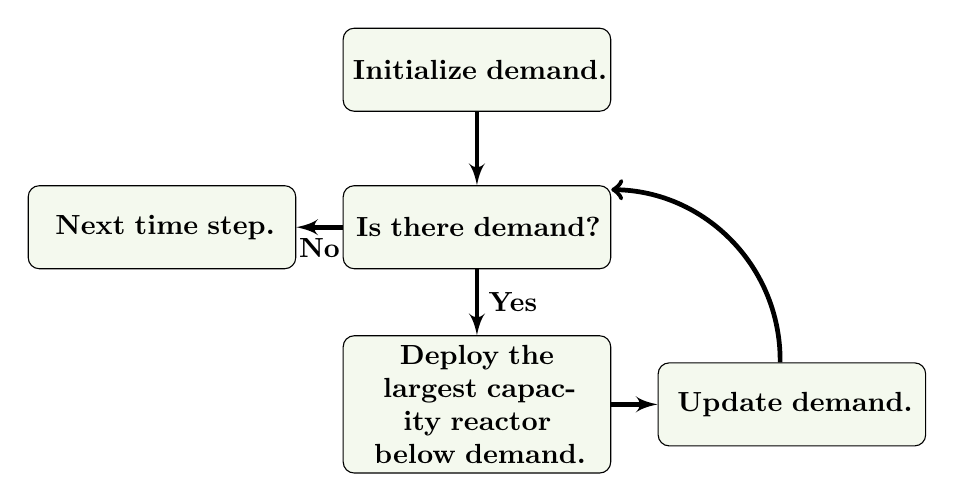
\begin{tikzpicture}[node distance = 2cm, auto]
        % Place nodes
        \node [block] (init) {\textbf{Initialize demand.}};
        \node [block, below of=init] (check) {\textbf{Is there demand?}};
        \node [block, below of=check, node distance=2.25cm] (evaluate) {\textbf{Deploy the largest capacity reactor below demand.}};
        % Draw edges
        \path [line, line width=0.6mm] (init) -- (check);
        \path [line, line width=0.6mm] (check) -- node {\textbf{Yes}} (evaluate); % \pause
        \node [block, right of=evaluate, node distance=4cm] (update) {\textbf{Update demand.}};
        \node [block, left of=check, node distance=4cm] (stop) {\textbf{Next time step.}};
        \path [line, line width=0.6mm] (evaluate) -- (update);
        \path [line, line width=0.6mm] (check) -- node {\textbf{No}}(stop);
        \draw[->, line width=0.6mm] (update) edge[bend right=45] node[right]{} (check);
      \end{tikzpicture}
      \caption{The greedy deployment diagram demonstrates a preference for the larger power capacity reactors, and shows how the scheme could under-deploy if the remaining capacity is less than the size of the smallest reactor.}
      \label{fig:greedy_diagram}
    \end{figure}
  \end{frame}

  \begin{frame}
    \frametitle{Random reactor deployment algorithm}
  % %   \begin{algorithm}[H]
  % %     \caption{Random Reactor Deployment Algorithm}
  %     \begin{algorithmic}[1]
  %         \State Initialize demand
  %         \While{demand exists}
  %             \State Randomly deploy a reactor that does not exceed demand
  %             \State Update demand
  %         \EndWhile
  %     \end{algorithmic}
  % %     \end{algorithm}
  \begin{figure}[H]
    \centering
    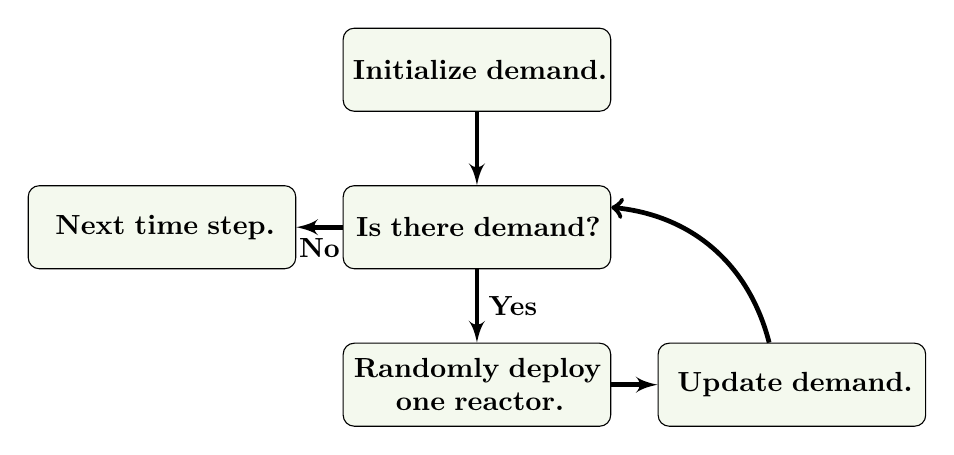
\begin{tikzpicture}[node distance = 2cm, auto]
      % Place nodes
      \node [block] (init) {\textbf{Initialize demand.}};
      \node [block, below of=init] (check) {\textbf{Is there demand?}};
      \path [line, line width=0.6mm] (init) -- (check); % \pause

      \node [block, below of=check, node distance=2cm] (evaluate) {\textbf{Randomly deploy one reactor.}};
      \path [line, line width=0.6mm] (check) -- node {\textbf{Yes}} (evaluate); % \pause

      \node [block, right of=evaluate, node distance = 4cm] (update) {\textbf{Update demand.}};
      \path [line, line width=0.6mm] (evaluate) -- (update); % \pause

      \draw[->, line width=0.6mm] (update) edge[bend right=35] node[right]{} (check); % \pause

      \node [block, left of=check, node distance=4cm] (stop) {\textbf{Next time step.}};
      \path [line, line width=0.6mm] (check) -- node {\textbf{No}}(stop);
    \end{tikzpicture}
    \caption{Random reactor deployment diagram. This algorithm randomly deploys reactors until the demand is met. If a reactor is deployed that exceeds the demand, it will simply be removed and the algorithm will try again.}
    \label{fig:random_diagram}
  \end{figure}
  \end{frame}

  \begin{frame}
    \frametitle{Random + greedy reactor deployment algorithm}
  % %     \begin{algorithm}[H]
  % %       \caption{Random + Greedy Reactor Deployment Algorithm}
  %       \begin{algorithmic}[1]
  %           \State Initialize demand
  %           \While{demand exists}
  %               \State Randomly deploy a reactor
  %               \If{demand is exceeded}
  %                   \State Remove last reactor
  %                   \If{demand still exists}
  %                       \State Select the largest reactor that does not exceed demand
  %                       \State Deploy until the next reactor exceeds demand
  %                       \State Update demand
  %                   \EndIf
  %               \EndIf
  %           \EndWhile
  %       \end{algorithmic}
  % %       \end{algorithm}
  \begin{figure}
    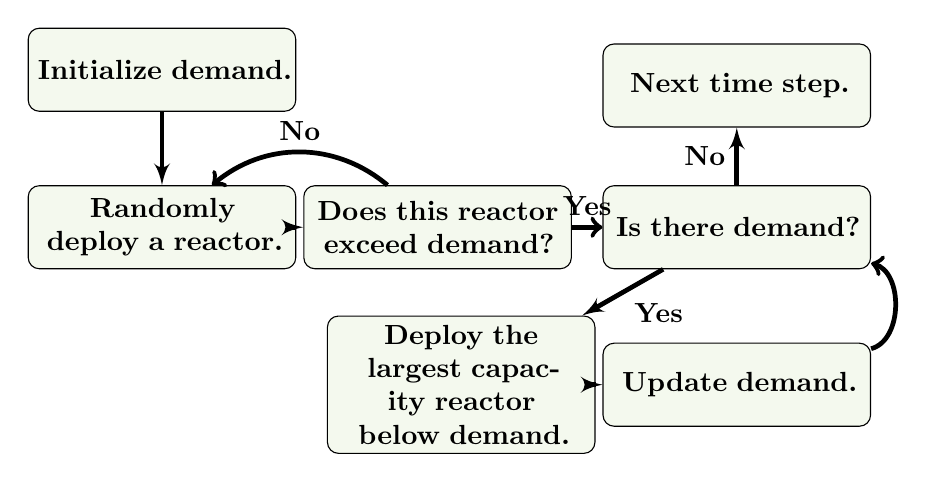
\begin{tikzpicture}[node distance = 2cm, auto]
      % Place random nodes
      \node [block] (init) {\textbf{Initialize demand.}};
      \node [block, below of=init, node distance=2cm] (evaluate) {\textbf{Randomly deploy a reactor.}};
      \node [block, right of=evaluate, node distance=3.5cm] (update) {\textbf{Does this reactor exceed demand?}};
      % Place greedy nodes
      \node [block, right of=update, node distance=3.8cm] (checkg) {\textbf{Is there demand?}};
      \node [block, below of=checkg, node distance=2cm] (updateg) {\textbf{Update demand.}};
      \node [block, left of=updateg, node distance=3.5cm] (evaluateg) {\textbf{Deploy the largest capacity reactor below demand.}};
      \node [block, above of=checkg, node distance=1.8cm] (stopg) {\textbf{Next time step.}};
      % Draw edges
      \path [line, line width=0.6mm] (init) -- (evaluate);
      \path [line, line width=0.6mm] (evaluate) -- (update);
      \draw[->, line width=0.6mm] (update) -- node[above]{\textbf{Yes}}(checkg);
      \draw[->, line width=0.6mm] (update) edge[bend right=40] node[above]{\textbf{No}} (evaluate);
      % Draw greedy edges
      \path [line, line width=0.6mm] (checkg) -- node {\textbf{Yes}} (evaluateg);
      \path [line, line width=0.6mm] (evaluateg) -- (updateg);
      \path [line, line width=0.6mm] (checkg) -- node[left] {\textbf{No}}(stopg);
      \draw[->, line width=0.6mm] (updateg) edge[bend right=75] node[right]{} (checkg);
  \end{tikzpicture}
  \caption{Random + Greedy deployment diagram. This algorithm first attempts to randomly deploy a reactor, and if that reactor exceeds demand, it will remove the last reactor and then use the greedy approach to fill in the remaining demand.}
  \label{fig:random_greedy_diagram}
  \end{figure}
  \end{frame}

  \section{LEU+ to HALEU}

  \begin{frame}
    \frametitle{Our demand for energy is going up}
    \begin{columns}
      \column{0.35\textwidth}
        We will compare each deployment algorithm with a demand growth scenario that:
        \begin{itemize}[<+->]
          \item doubles nuclear capacity by 2050,
          \item starts deploying the advanced reactors in 2030,
          \item and uses LEU+ from 2030-2040.
        \end{itemize}
      \column{0.65\textwidth}
        \begin{figure}
          \centering
          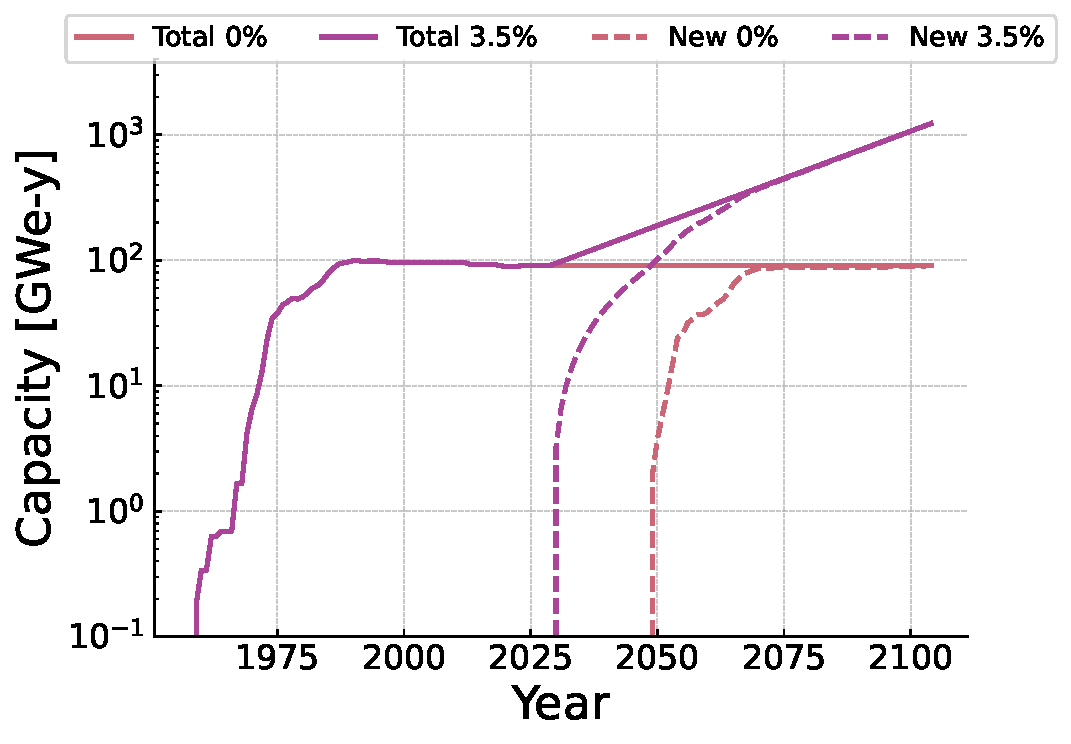
\includegraphics[width=\textwidth]{../images/new_capacity_ng_d2.pdf}
          \caption{Nuclear electricity capacity to present day with projection of doubling nuclear by 2050 from DOE Liftoff Report \cite{julie_liftoff_pathways_2024}.}
        \end{figure}
    \end{columns}
  \end{frame}

  \begin{frame}
    \frametitle{The total mass for scenarios with and without LEU+}
    We have approximated that each reactor's capacity for LEU+ will be the same as their capacity for HALEU.
    \begin{columns}
      \begin{column}{0.5\textwidth}
        \begin{figure}
          \centering
          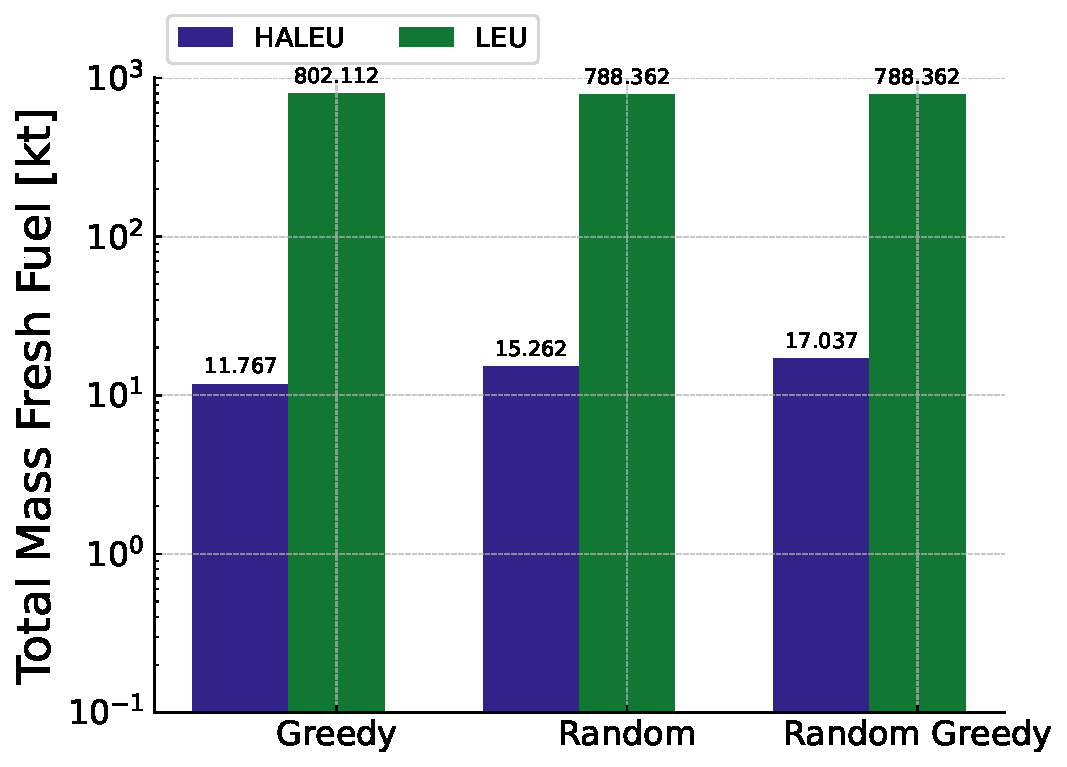
\includegraphics[width=\textwidth]{../images/final_cumulative_fuel_of.pdf}
          \caption{No-LEU+ scenario.}
        \end{figure}
      \end{column}
      \begin{column}{0.5\textwidth}
        \begin{figure}
          \centering
          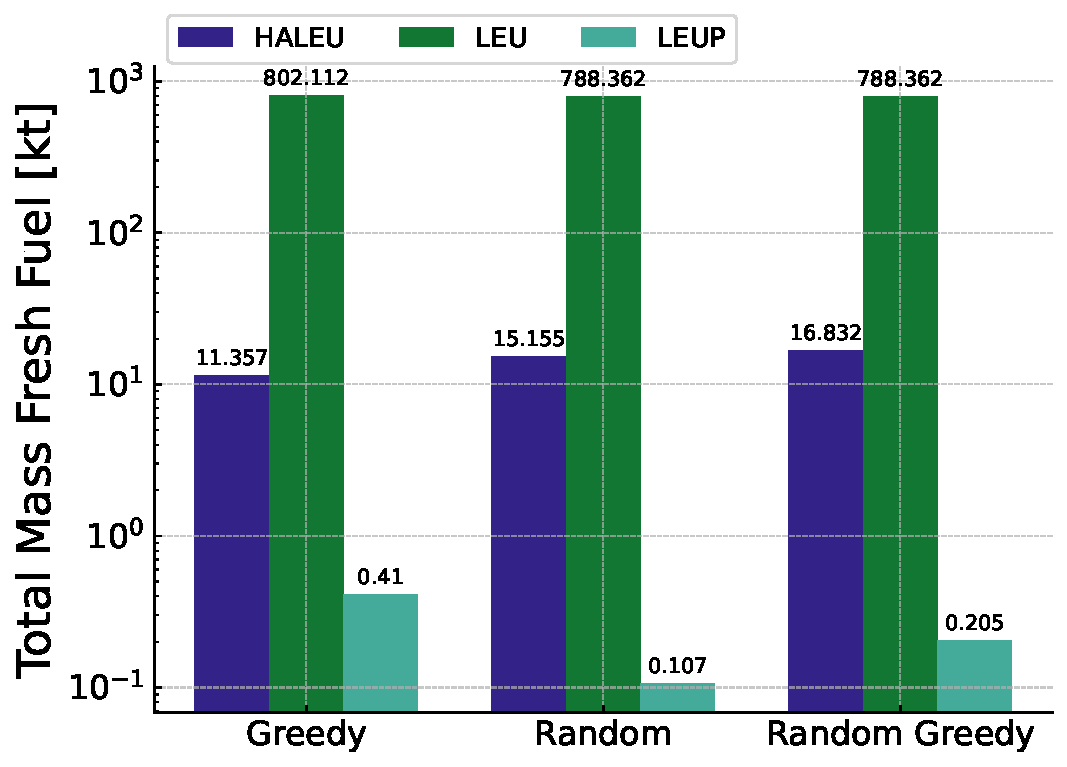
\includegraphics[width=\textwidth]{../images/final_cumulative_fuel_mf.pdf}
          \caption{LEU+ to HALEU scenario.}
        \end{figure}
      \end{column}
    \end{columns}
  \end{frame}

  \begin{frame}
    \frametitle{Comparing the mass of HALEU for each scenario}
    In our one-to-one scenario for LEU+- and HALEU-fueled reactors, the LEU+ scenarios require less HALEU on the order of hundreds of tonnes.
    \begin{figure}
        \centering
        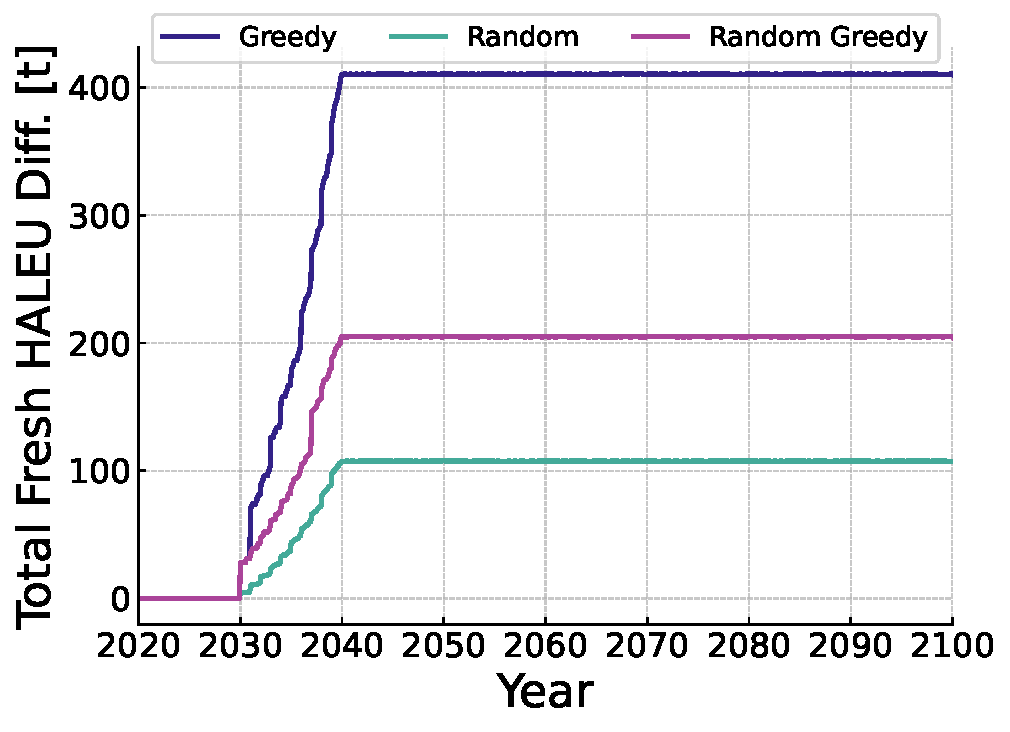
\includegraphics[width=0.65\textwidth]{../images/diff_scheme.pdf}
    \end{figure}
  \end{frame}

  \begin{frame}
    \frametitle{Breaking down the mass of HALEU by reactor}
    We can separate the differences in HALEU between the LEU+ and non-LEU+ scenarios by reactor for each deployment algorithm to show that the larger differences are for the Xe-100.
    \begin{figure}
      \centering
      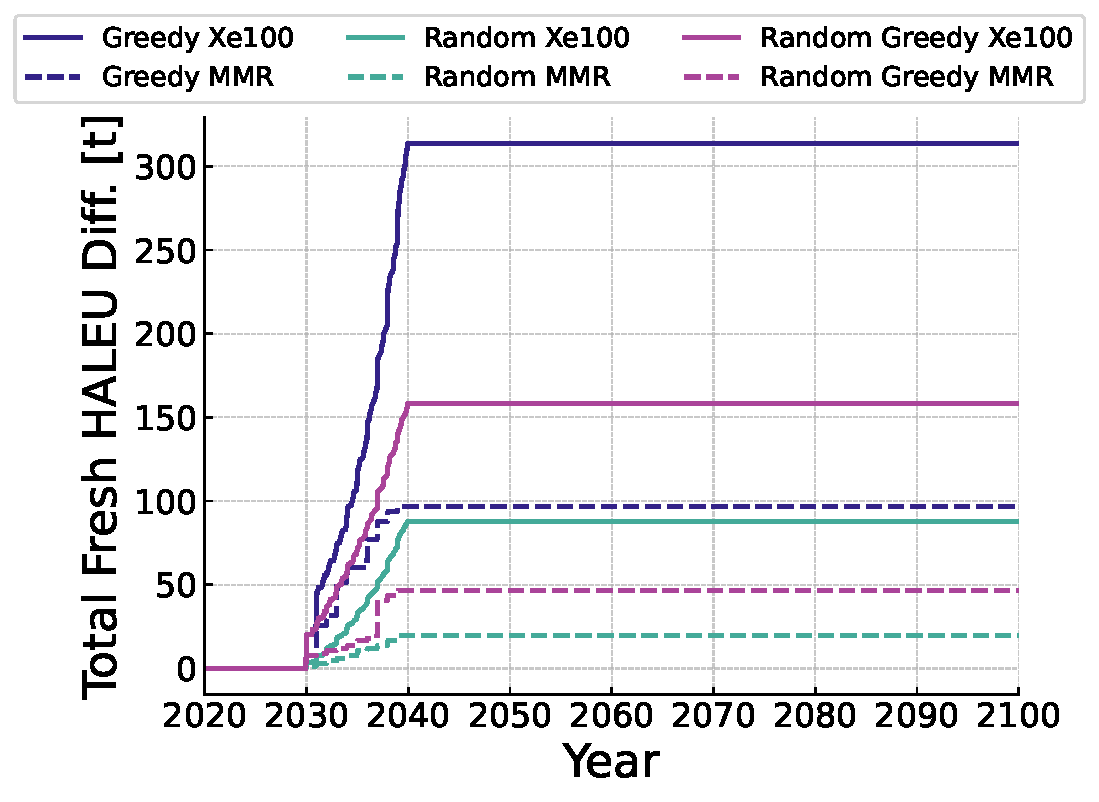
\includegraphics[width=0.7\textwidth]{../images/diff_reactor_fuel.pdf}
    \end{figure}
  \end{frame}


  \section{Conclusion}
  \begin{frame}
      \frametitle{This is an upperbound on the amount of HALEU we could defer.}
      In our simple case, we transition from LEU+ to HALEU after 10 years of operation with no learning curve.
      \begin{itemize}
          \item For the Xe100 reactors, we need almost 315 less tons of HALEU.
          \item For the MMR reactors, we need almost 97 less tons of HALEU.
      \end{itemize}
  \end{frame}

  \begin{frame}
    \frametitle{Future work}
    We are interested in:
    \begin{itemize}
      \item adapting neutronics models of the MMR and Xe-100 to be fueled with LEU+,
      \item investigating the impact of learning curves instead of a ready deployment on the results over time,
      \item and comparing these results with a triple-by-2050 scenario (also proposed in the Liftoff Report \cite{julie_liftoff_pathways_2024}).
    \end{itemize}
  \end{frame}


  \begin{frame}
    \frametitle{Acknowledgement}
      % This research was performed, in part, using funding received from the DOE
      % Office of Nuclear Energy's Nuclear Energy University Program (Project 23-29656
      % DE-NE0009390) 'Illuminating Emerging Supply Chain and Waste Management
      % Challenges'.


      Thanks to Luke Seifert for his help with running the neutronics models, and thanks to Amanda Bachmann and Zoe Richter for letting me adapt their reactor models for the MMR and Xe100.

      \vspace{7mm}
      As always, thanks to my advisors Madicken Munk and Katy Huff for their support throughout my studies.
  \end{frame}


%%--------------------------------%%
%%--------------------------------%%
\begin{frame}[allowframebreaks]
  \frametitle{References}
  \bibliographystyle{IEEEtran}
  {\footnotesize \bibliography{../bibliography.bib} }

\end{frame}

\appendix

 \begin{frame}
    \frametitle{We define the enrichment levels as...}
    \begin{table}[H]
        \centering
        \caption{Enrichment levels and their ranges.}
        \label{tab:enrichment_levels}
        \begin{tabular}{l l}
           \hline
           \textbf{Enrichment Level} & \textbf{Range [\%  $^{235}$U]} \\
           \hline
           Natural & $<$ 0.711 \\
           LEU & 0.711-5 \\
           LEU+ & 5-10 \\
           HALEU & 10-20 \\
           HEU & $\geq$ 20  \\
           \hline
        \end{tabular}
     \end{table}
     \vspace{8pt}
     These are a mash-up of economic and regulatory definitions.
  \end{frame}

\begin{frame}
  \frametitle{Staggering enrichment could give the supply chain time to form}
  \begin{figure}
      \centering
      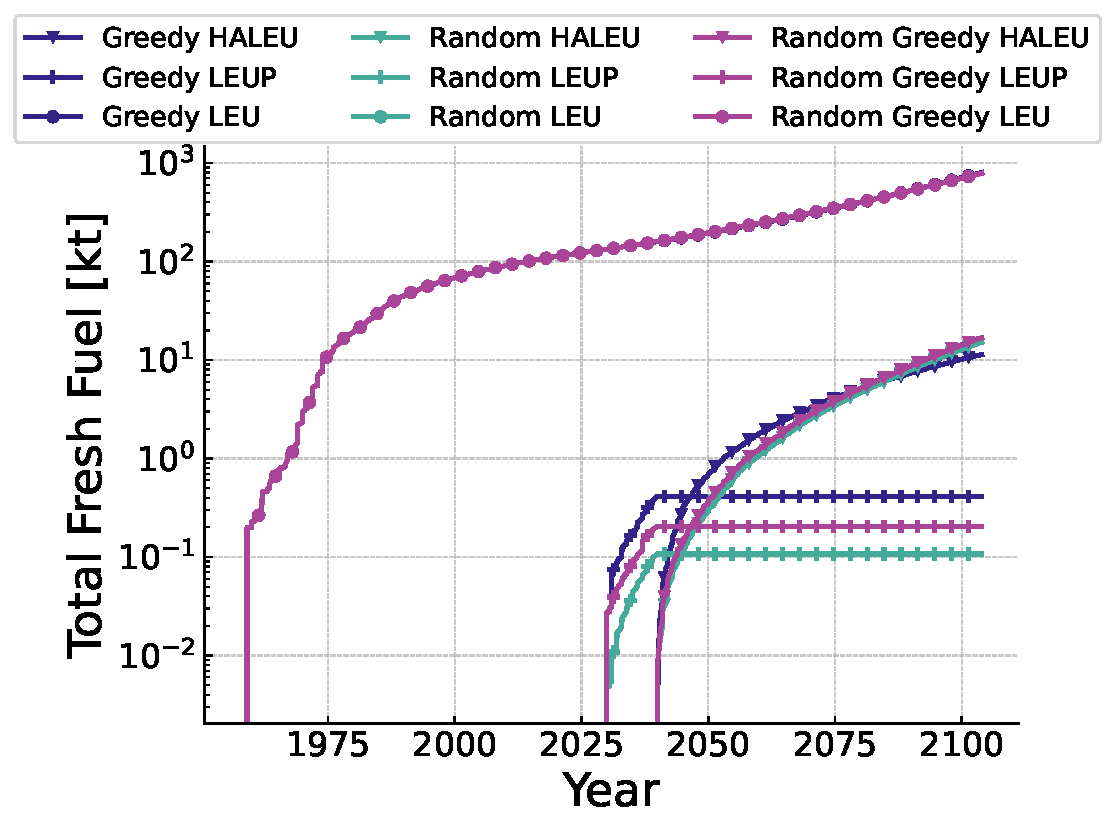
\includegraphics[width=0.85\textwidth]{../images/total_fuel_over_time.pdf}
  \end{figure}
\end{frame}

\begin{frame}
  \frametitle{The differences between LEU demand are small in kt}
  \begin{figure}
      \centering
      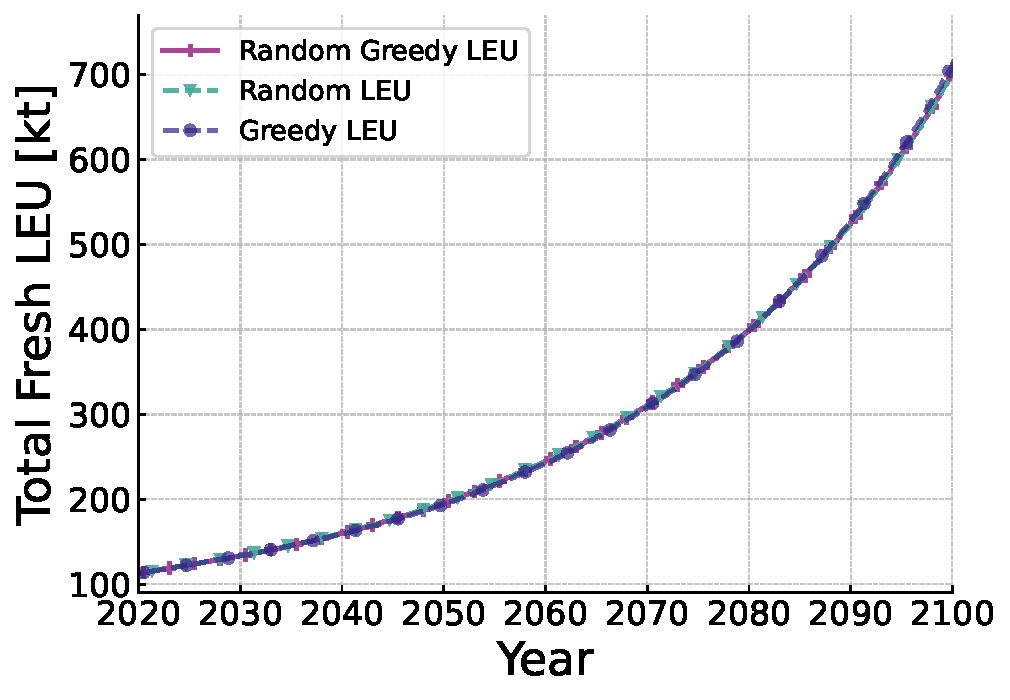
\includegraphics[width=0.85\textwidth]{../images/total_leu_over_time.pdf}
  \end{figure}
\end{frame}
%%--------------------------------%%


\end{document}



